\documentclass[a4paper, oneside, 12pt]{article}

\usepackage{../custom}

\usepackage[backend=biber]{biblatex}
\addbibresource{biblio.bib}

\title{Annexe}
\author{Groupe 1225}
\date{\today}

\begin{document}

\maketitle

\section{Résultats des simulations sur \textsc{Aspen Plus}}
Nous regroupons ici tous les résultats produits par nos simulations réalisées sur le programme \textsc{Aspen Plus}. Pour chacune d'elles, nous précisons le modèle utilisé ainsi que les conditions dans le réacteur et la fraction purgée du recyclage. On accorde en particulier de l'attention aux résultats concernant les flux sortants: \textsc{NH3,OUT} et \textsc{PURGE}.

\graphicspath{{Img_simulations/}}

\begin{figure}[h!]
	\begin{center}
		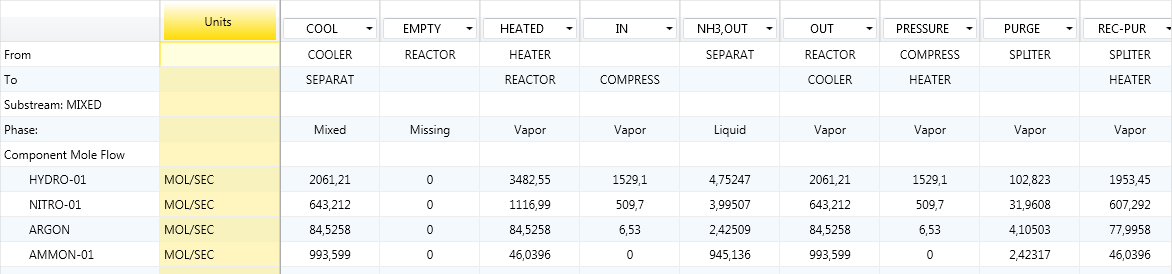
\includegraphics[scale=0.5]{RK-ASPEN.png}
	\end{center}
	\caption{Modèle \texttt{RK-ASPEN}, 750 K, 270 bar, 5\%}
	\label{fig:RK-ASPEN}
\end{figure}


\begin{figure}[h!]
	\begin{center}
		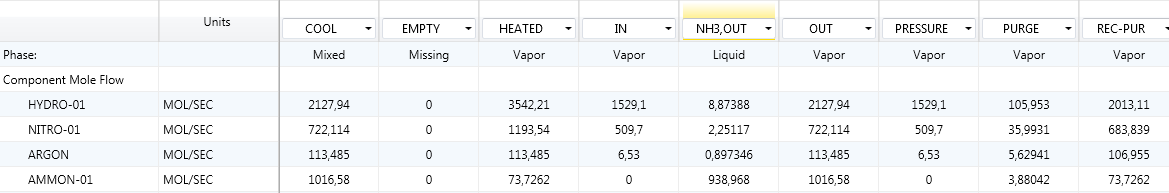
\includegraphics[scale=0.5]{PSRK.png}
	\end{center}
	\caption{Modèle \texttt{PSRK}, 750 K, 270 bar, 5\%}
	\label{fig:PSRK}
\end{figure}

\begin{figure}[h!]
	\begin{center}
		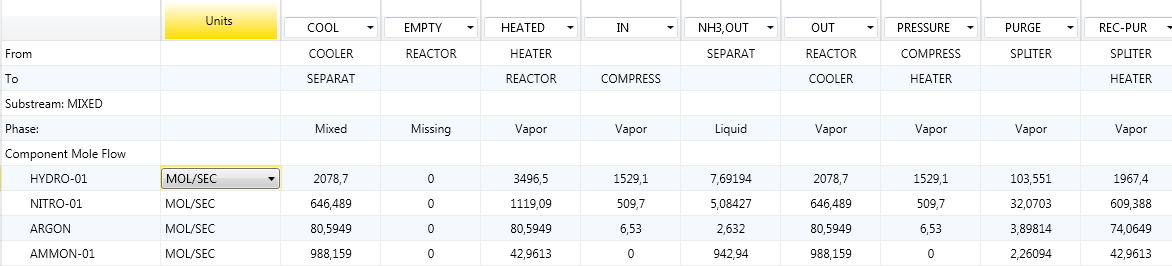
\includegraphics[scale=0.5]{SRK,750,270,5.png}
	\end{center}
	\caption{Modèle \texttt{SRK}, 750 K, 270 bar, 5\%}
	\label{fig:SRK,750,270,0.05}
\end{figure}

\begin{figure}[h!]
	\begin{center}
		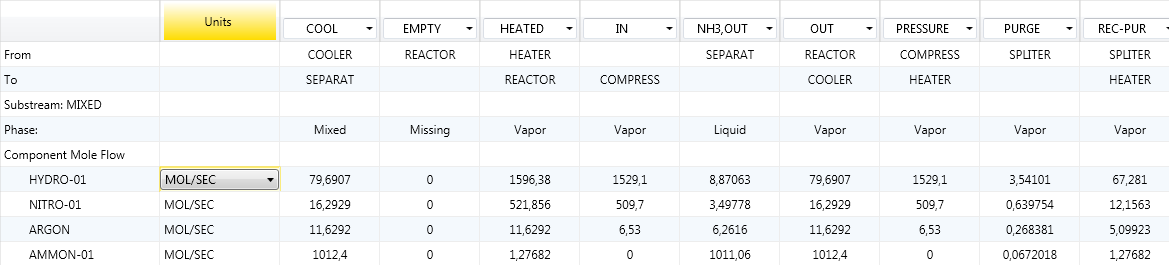
\includegraphics[scale=0.5]{SRK,500,270.png}
	\end{center}
	\caption{Modèle \texttt{SRK}, 500 K, 270 bar, 5\%}
	\label{fig:SRK,500,270,0.05}
\end{figure}

\begin{figure}[h!]
	\begin{center}
		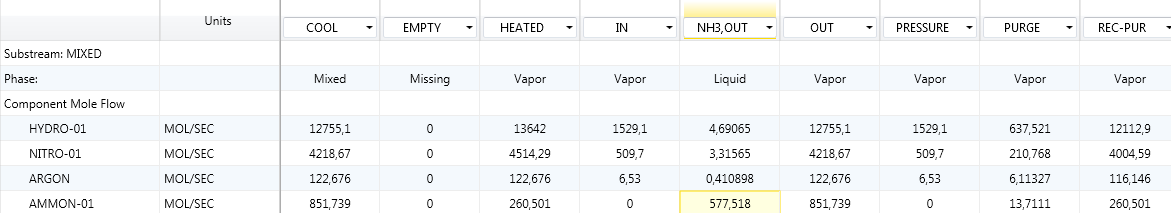
\includegraphics[scale=0.5]{SRK,1000,270.png}
	\end{center}
	\caption{Modèle \texttt{SRK}, 1000 K, 270 bar, 5\%}
	\label{fig:SRK,1000,270,0.05}
\end{figure}

\begin{figure}[h!]
	\begin{center}
		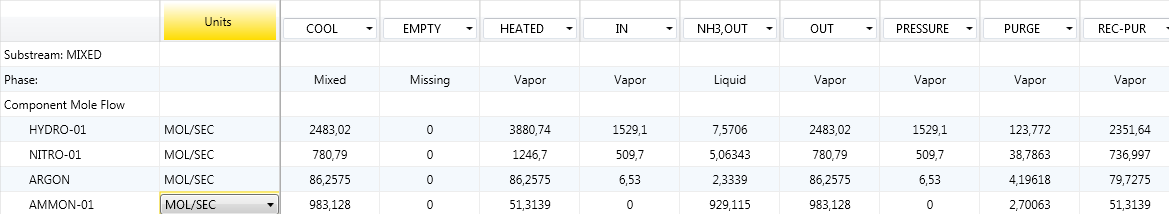
\includegraphics[scale=0.5]{SRK,750,220.png}
	\end{center}
	\caption{Modèle \texttt{SRK}, 750 K, 220 bar, 5\%}
	\label{fig:SRK,750,220,0.05}
\end{figure}

\begin{figure}[h!]
	\begin{center}
		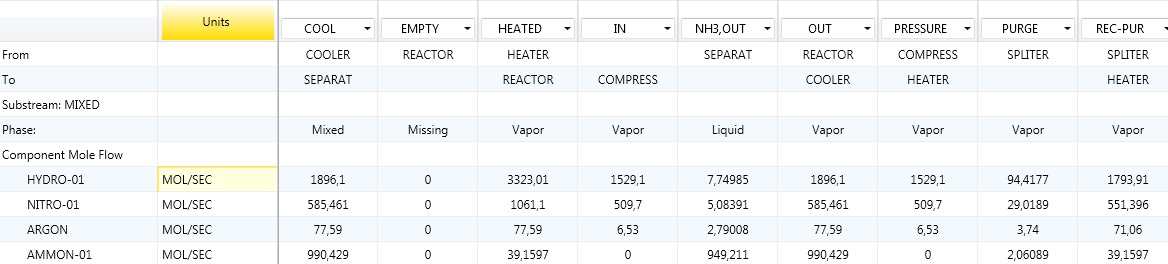
\includegraphics[scale=0.5]{SRK,750,300.png}
	\end{center}
	\caption{Modèle \texttt{SRK}, 750 K, 300 bar, 5\%}
	\label{fig:SRK,750,300,0.05}
\end{figure}

\begin{figure}[h!]
	\begin{center}
		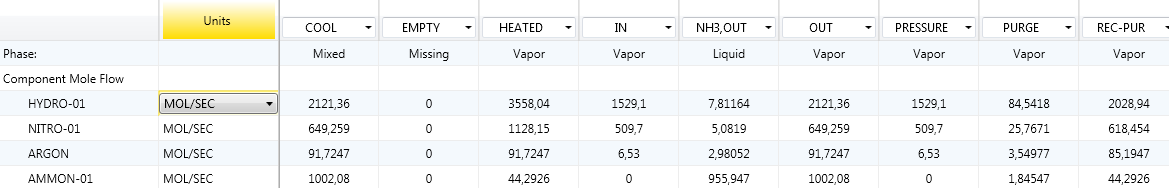
\includegraphics[scale=0.5]{SRK,750,270,4.png}
	\end{center}
	\caption{Modèle \texttt{SRK}, 750 K, 270 bar, 4\%}
	\label{fig:SRK,750,270,0.04}
\end{figure}

\begin{figure}[h!]
	\begin{center}
		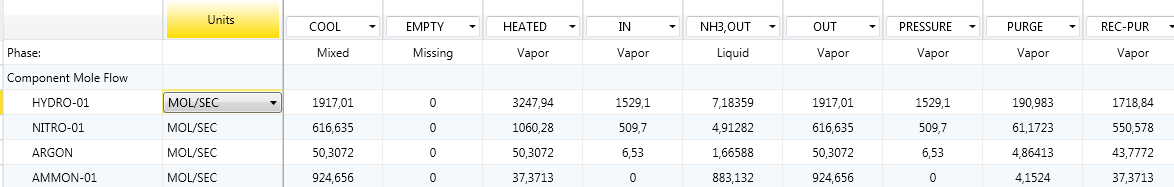
\includegraphics[scale=0.5]{SRK,750,270,10.png}
	\end{center}
	\caption{Modèle \texttt{SRK}, 750 K, 270 bar, 10\%}
	\label{fig:SRK,750,270,0.1}
\end{figure}

\begin{figure}[h!]
	\begin{center}
		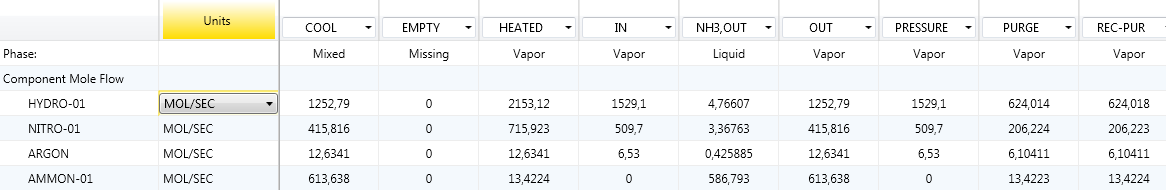
\includegraphics[scale=0.5]{SRK,750,270,50.png}
	\end{center}
	\caption{Modèle \texttt{SRK}, 750 K, 270 bar, 50\%}
	\label{fig:SRK,750,270,0.5}
\end{figure}

\begin{figure}[h!]
	\begin{center}
		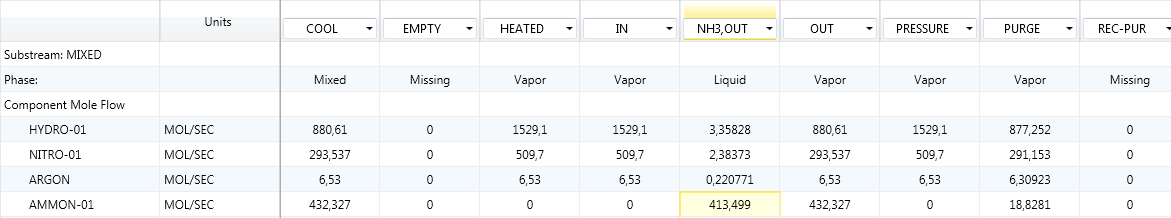
\includegraphics[scale=0.5]{SRK,750,270,100.png}
	\end{center}
	\caption{Modèle \texttt{SRK}, 750 K, 270 bar, 100\%}
	\label{fig:SRK,750,270,1}
\end{figure}

\section{Outil de calcul: codes \textsc{Matlab}}

\end{document}

